\section{Impacto das Condições de Captura ($H_2$ e $H_3$)}

Nesta seção, isolamos as variáveis de iluminação física e pré-processamento digital para validar as hipóteses $H_2$ e $H_3$.

\subsection{Impacto da Iluminação ($H_2$)}
A evolução do MCC através das diferentes fontes de luz (AB, AM, BR) é ilustrada na Figura \ref{fig:h2_lighting}. Observa-se um crescimento consistente na performance à medida que a iluminação é otimizada fisicamente, culminando na versão BR (V10). Este resultado confirma $H_2$, demonstrando que a qualidade do sinal físico de entrada é um preditor de sucesso mais forte que a complexidade algorítmica isolada.

\begin{figure}[h!]
  \centering
  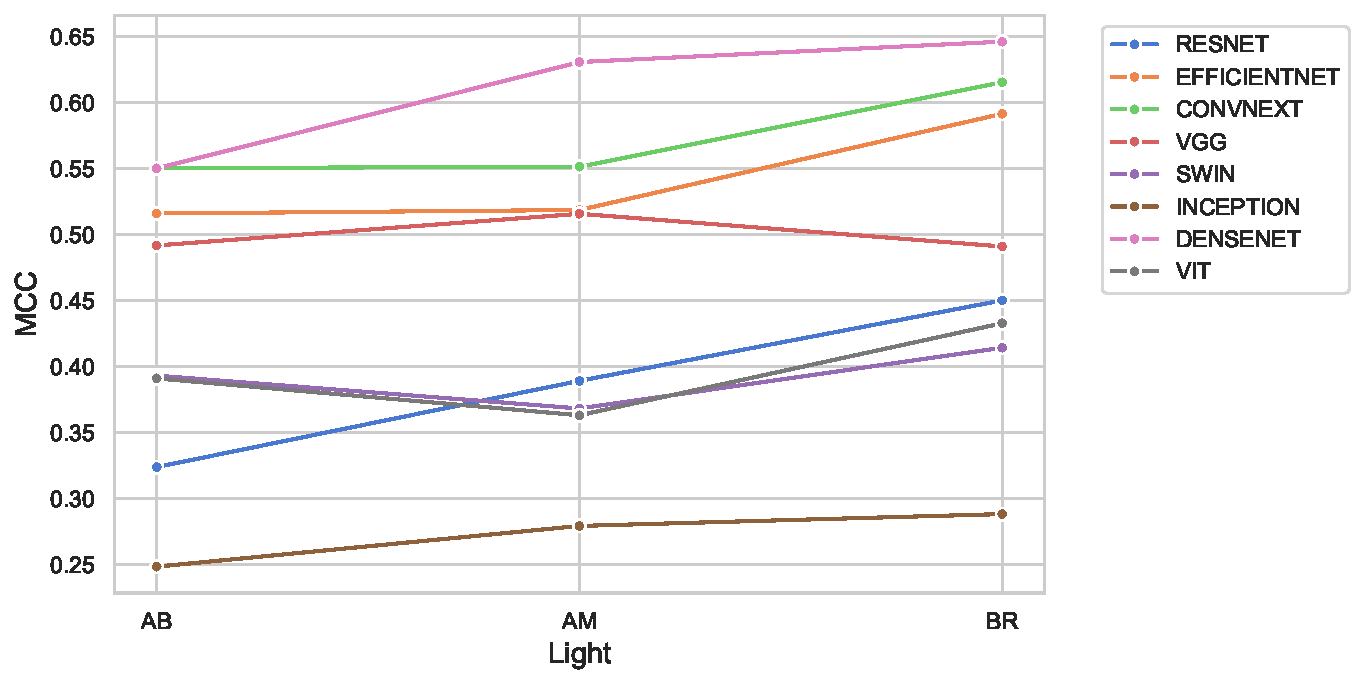
\includegraphics[width=0.8\textwidth]{images/h2_lighting_impact.pdf}
  \caption{Impacto da Iluminação ($H_2$): Evolução do MCC para cada modelo conforme a fonte de luz é otimizada.}
  \label{fig:h2_lighting}
\end{figure}

\subsection{Expansão Espectral via Engenharia de Features ($H_3$)}
Em contraste, a tentativa de auxiliar os modelos via expansão espectral artesanal (15 canais Gabor) na versão \textbf{V8} resultou em uma degradação severa, como mostrado na Figura \ref{fig:h3_spectral}. Este achado refuta $H_3$, indicando que para classificadores profundos, a inserção de \textit{features} pré-computadas ruidosas pode atuar como um mecanismo de confusão no aprendizado \textit{end-to-end}.

\begin{figure}[h!]
  \centering
  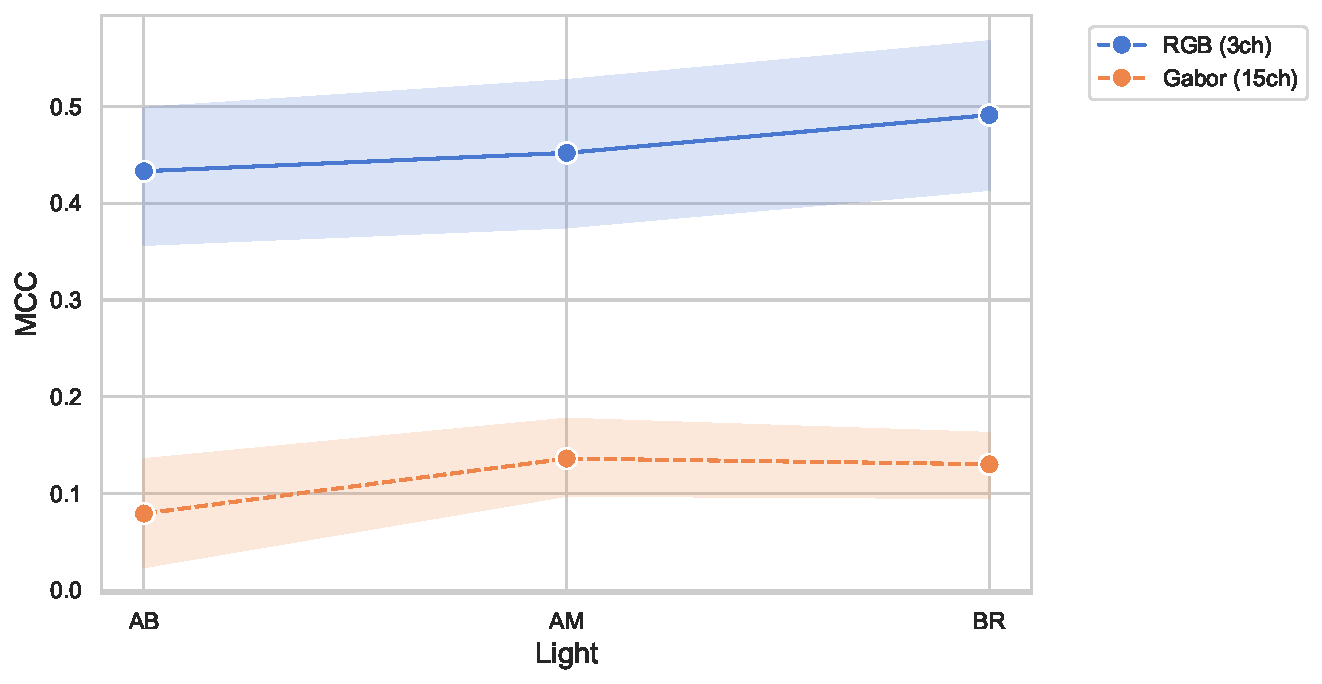
\includegraphics[width=0.8\textwidth]{images/h3_spectral_impact.pdf}
  \caption{Falha da Expansão Espectral ($H_3$): O contraste entre a V1 (RGB) e a V8 (15-canais) mostra a queda drástica de performance.}
  \label{fig:h3_spectral}
\end{figure}
